
\subsection{Comportamientos e implementaciones}
\label{comportamientos}

Una vez que decidimos utilizar la arquitectura explicada en la secci\'on \ref{arq_prop}
para nuestro proyecto, tuvimos que analizar:
\begin{itemize}
\item{}Forma de implementaci\'on de la arquitectura en c\'odigo
\item{}Comportamientos a realizar
\item{}Ordenes de inhibici\'on y supresi\'on entre los mismos
\item{}Forma de implementaci\'on de los mismos
\item{}Orden de implementaci\'on
\end{itemize}

%Detallar que se hizo con cada item
Para implementar la arquitectura decidimos asignarle un $ID$ num\'erico diferente a cada comportamiento.
Tambi\'en tomamos la decisi\'on de elegir como comportamiento activo en el instante $t$,
aquel comportamiento que est\'e activo en ese instante y tenga mayor $ID$,
suprimiendo as\'i el resto de los comportamientos ( con un $ID$ menor ) que podr\'ian estar activos.

%Explicar como se relaciona el requerimiento (robot recolector de basura autonomo) con los comportamientos que pusimos
El requerimiento de este proyecto es la realizaci\'on de un robot aut\'onomo que recolecte
basura de su entorno din\'amico pero estructuralmente fijo. De aqu\'i se infieren algunos de los
comportamientos que debe tener el robot:
\begin{itemize}
	\item{\emph{Recolectar basura} (\ref{collect_garbage})}
	\item{\emph{Recargar bater\'ia} (\ref{recharge_battery}):} Por ser aut\'onomo, debe poder 
			ser capaz de recargarse s\'olo para poder continuar con su actividad.
	\item{\emph{Wandering} (\ref{wandering}):} El robot no es controlado por control, ya que
			es aut\'onomo, por lo que debe poder recorrer el entorno por s\'i mismo.
	\item{\emph{Evitamiento de obst\'aculos} (\ref{avoid_obstacles}):} Debido a la naturaleza del
			entorno, el robot debe ser capaz de navegar sin chocarse contra los l\'imites del entorno
			ni con las personas que circulan por el mismo.
\end{itemize}

El comportamiento de recolectar basura y el requerimiento de la autonom\'ia llevan a su vez
a la aparici\'on de m\'as comportamientos: \emph{Descargar basura} (\ref{unload_garbage})
e \emph{Ir hacia basura} (\ref{go_to_garbage}).
\\
La figura \ref{fig:architecture} muestra los comportamientos implementados y su orden de jerarqu\'ia.
Se puede ver que hay m\'as comportamientos de los detallados anteriormente. \'Esto se debi\'o a que la forma
en que se implementamos los comportamientos b\'asicos del robot nos requiri\'o el desarrollo
de comportamientos auxiliares.
\\
\begin{figure}[htp]
\begin{center}
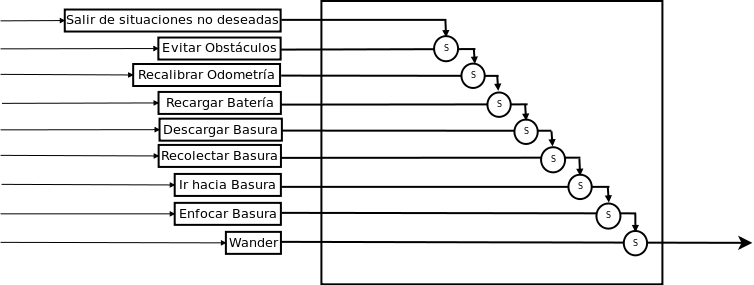
\includegraphics[scale=0.5]{comportamientos/behavioursArchitecture.png}
\caption{Arquitectura de Comportamientos}
\label{fig:architecture}
\end{center}
\end{figure}
\\
Primero implementamos \emph{Wandering} debido a, en una primera aproximaci\'on, la sencillez
del mismo. Luego implementamos \emph{Evitamiento de obst\'aculos} para lograr que el robot pueda
navegar sin problemas por el arena. Como el comportamiento de recolectar e ir hacia la basura
dependend\'ia del m\'odulo de reconocimiento de objetos y el mismo estaba siendo desarrollado
en paralelo, se decidi\'o implementar el comportamiento de \emph{Recargar bater\'ia} y \emph{Descargar basura}.
Una vez que tuvimos la primera implementaci\'on funcional del reconomiento de objetos, procedimos a
desarrollar \emph{Ir hacia basura} y \emph{Recolectar Basura}.
\\
A continuaci\'on detallamos los comportamientos indicados en la figura \ref{fig:architecture},
as\'i como la implementaci\'on en \textit{pseudo-codigo} de los mismos y detalles tenidos
en cuenta para la realizaci\'on de los mismos.
%A continuacion vamos a explicar cada comportamiento.....

\subsubsection{Wandering}
\label{wandering}

\paragraph{Detalle del comportamiento} 
Por ser el comportamiento que menor jerarqu\'ia tiene (Ver \ref{fig:architecture}), es el \'unico
comportamiento que est\'a activado ante la ausencia de un est\'imulo, asegurandonos que siempre
haya por lo menos un comportamiento activo.
\\
En una primer aproximaci\'on de \emph{Wandering}, s\'olo nos preocupamos por ir hacia adelante
ya que eventualmente, el robot encuentra un obst\'aculo y realiza un giro cambiando la direcci\'on
del robot.
\\
Los resultados de la simulaci\'on nos indicaron que el robot no recorr\'ia ciertas zonas o las recorr\'ia
despu\'es de un largo tiempo, lo que nos llev\'o a un segundo approach. El mismo tiene en cuenta el hecho
de que el robot posee una c\'amara y por lo tanto se puede llevar un seguimiento de los lugares que m\'as
recientemente visit\'o o las zonas que hace mucho tiempo no visita.
\\
\'Este approach, en cierta forma, genera un modelo del mundo, un hecho que conflict\'ua con uno de
los principios propuestos a seguir en la secci\'on \ref{arq_prop}. Para minimizar el conflicto, decidimos
mantener al m\'inimo la informaci\'on almacenada para el funcionamiento del algoritmo, es decir, por cada
zona de arena s\'olo mantenemos el timestamp de la \'ultima vez que el robot la visit\'o.

\paragraph{Implementaci\'on del comportamiento}

La implementaci\'on del segundo approach, en \emph{pseudo-c\'odigo} es la siguiente:
\begin{verbatim}
por cada paso
    zona = pedir_zona_vista(camara)
    marcar_zona_como_vista(modelodelmundo,zona)
    ultimazonavisitada = pedir_ultima_zona_visitada(modelodelmundo)
    velocidades = calcular_velocidades_de_ruedas(ultimazonavisitada)
    poner_velocidades_en_ruedas(velocidades)
\end{verbatim}
Para obtener la zona vista por la c\'amara, necesitamos de la altura $c_h$ a la cual est\'a ubicada
la c\'amara en el robot, el campo de visi\'on (de ahora en adelante \emph{Field of View o FOV})
horizontal $FOV_h$ o vertical $FOV_v$ y el \'angulo de inclinaci\'on de la c\'amara $ac$. Viendo la figura
\ref{fig:angleCamera} podemos ver que:

\begin{eqnarray}
ac + \frac{FOV_v}{2} + \theta = \frac{\pi}{2}\\
\gamma + FOV_v + \theta = \frac{\pi}{2}\\
\tan(\gamma) = \frac{d}{c_h}\\
\tan(\gamma+FOV_v) = \frac{d+h}{c_h}
\end{eqnarray}

%En caso de no disponer del $FOV_v$, el mismo se puede obtener de:
%\begin{equation}
%FOV_v = \atan(\frac{ \tan(\frac{FOV_h}{2}) * height}{width} * 2)\\
%\end{equation}
Organizando las ecuaciones, podemos deducir que:

\begin{eqnarray}
\gamma = \frac{\pi}{2} + ac - \frac{FOV_v}{2}\\
d = \tan(\gamma) * c_h \\
d+h = \tan(\gamma+FOV_v) * c_h
\end{eqnarray}

Por lo que obtenemos el \'angulo hasta el inicio de la im\'agen de la c\'amara $\gamma$ y como consecuencia,
la distancia $d$ desde la posici\'on de la c\'amara hasta el inicio de la im\'agen y $d+h$,
la distancia desde la posici\'on de la c\'amara hasta el final de la im\'agen. Usando \'estos
datos, la posici\'on del robot $P$ y bas\'andonos en la figura \ref{fig:zoneCamera}, podemos obtener
los puntos $A$, $B$, $C$ y $D$ del trapezoide que determina la zona que ve la c\'amara.

\begin{figure}[htp]
\begin{center}
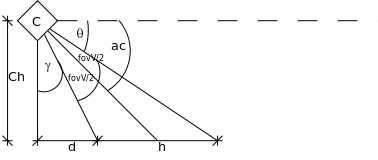
\includegraphics{comportamientos/angleCamera.png}
\caption{Diagrama de posici\'on de la c\'amara}
\label{fig:angleCamera}
\end{center}
\end{figure}

\begin{figure}[htp]
\begin{center}
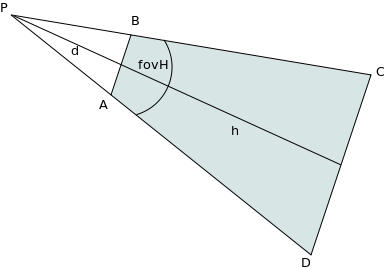
\includegraphics{comportamientos/rectangleWander.png}
\caption{Zona vista por la c\'amara}
\label{fig:zoneCamera}
\end{center}
\end{figure}

\subsubsection{Enfocar Basura}
\emph{Enfocar basura} surge como una necesidad ante la elecci\'on de la forma en que se va a la basura.
\label{focus_garbage}
\paragraph{Detalle del comportamiento}
la elecci\'on de la forma en que se va a la basura.
\paragraph{Implementaci\'on del comportamiento}

\subsubsection{Ir a Basura}
\label{go_to_garbage}
\paragraph{Detalle del comportamiento}
\paragraph{Implementaci\'on del comportamiento}

\subsubsection{Recolectar Basura}
\label{collect_garbage}
\paragraph{Detalle del comportamiento}
\paragraph{Implementaci\'on del comportamiento}

\subsubsection{Ir a zona de descarga de basura}
\label{go_to_unload_zone}

\paragraph{Buscar l\'inea}
\label{find_line}
\subparagraph{Detalle del comportamiento}
\subparagraph{Implementaci\'on del comportamiento}

\paragraph{Entrar a l\'inea}
\label{enter_line}
\subparagraph{Detalle del comportamiento}
\subparagraph{Implementaci\'on del comportamiento}

\paragraph{Seguir l\'inea}
\label{follow_line}
\subparagraph{Detalle del comportamiento}
\subparagraph{Implementaci\'on del comportamiento}

\subsubsection{Descargar Basura}
\label{unload_garbage}
\paragraph{Detalle del comportamiento}
\paragraph{Implementaci\'on del comportamiento}

\subsubsection{Ir a base de recarga de bater\'ia}
\label{go_to_recharge}
\paragraph{Detalle del comportamiento}
\paragraph{Implementaci\'on del comportamiento}

\subsubsection{Cargar Bater\'ia}
\label{recharge_battery}
\paragraph{Detalle del comportamiento}
\paragraph{Implementaci\'on del comportamiento}

\subsubsection{Recalibrarse}
\label{recalibrate}
\paragraph{Detalle del comportamiento}
\paragraph{Implementaci\'on del comportamiento}

\subsubsection{Evitar Obst\'aculos}
\label{avoid_obstacles}
\paragraph{Detalle del comportamiento}
\paragraph{Implementaci\'on del comportamiento}

\subsubsection{Salir de situaciones no deseadas}
\label{out_of_unwanted_situations}
\paragraph{Detalle del comportamiento}
\paragraph{Implementaci\'on del comportamiento}

